\chapter{Advanced Multi Head Attention}
Questo capitolo esplora le tecniche avanzate di attenzione multi-head, analizzando le ottimizzazioni che hanno reso possibile l'implementazione efficiente dei modelli di linguaggio di grandi dimensioni. Vengono trattate le tecniche di caching KV, le varianti Multi Query Attention (MQA) e Grouped Query Attention (GQA), gli embeddings posizionali rotatori (RoPE) e la recente Multi Head Latent Attention (MLA). Ogni tecnica viene presentata con le sue motivazioni teoriche, implementazioni pratiche e impatti sulle prestazioni.


\section{Introduzione}

L'architettura Transformer ha rivoluzionato il campo del deep learning per il processamento del linguaggio naturale. Tuttavia, con l'aumento delle dimensioni dei modelli e delle sequenze di input, l'efficienza computazionale e di memoria del meccanismo di attenzione multi-head è diventata una sfida critica. Adesso esploreremo le tecniche avanzate sviluppate per ottimizzare l'attenzione, mantenendo o migliorando le prestazioni dei modelli.

\section{KV Cache}

Durante la fase di inferenza nei modelli autoregressivi, il calcolo dell'attenzione per ogni nuovo token richiede l'accesso alle rappresentazioni di tutti i token precedenti. Senza ottimizzazioni, questo comporterebbe il ricalcolo completo delle matrici Key (K) e Value (V) per ogni posizione ad ogni step di generazione. La tecnica del \textbf{KV Cache} risolve questo problema memorizzando le matrici Key e Value calcolate nei passi precedenti:

\begin{equation}
\text{Attention}(Q_t, K_{1:t}, V_{1:t}) = \text{softmax}\left(\frac{Q_t K_{1:t}^T}{\sqrt{d_k}}\right) V_{1:t}
\end{equation}

dove $Q_t$ è la query per il token corrente alla posizione $t$, mentre $K_{1:t}$ e $V_{1:t}$ rappresentano tutte le chiavi e valori dalla posizione 1 alla posizione $t$.

\subsection{Implementazione del Cache}
Ad ogni step di generazione:
\begin{enumerate}
\item Si calcola la nuova coppia key-value per il token corrente;
\item Si concatena questa coppia al cache esistente;
\item Si utilizza il cache aggiornato per calcolare l'attenzione.
\end{enumerate}

Questo approccio riduce la complessità temporale da $o(T^2)$ a $o(T)$ per ogni nuovo token, dove $T$ è la lunghezza della sequenza.

\subsection{Requisiti di Memoria}
La dimensione del KV Cache per un layer di attenzione multi-head standard è:

\begin{equation}
\text{Cache Size} = 2 \times \text{batch\_size} \times \text{num\_heads} \times \text{seq\_length} \times \text{head\_dim}
\end{equation}

Il fattore 2 deriva dalla necessità di memorizzare sia le matrici Key che Value. Questa crescita lineare con la lunghezza della sequenza rappresenta una limitazione significativa per sequenze molto lunghe.

\begin{figure}
    \centering
    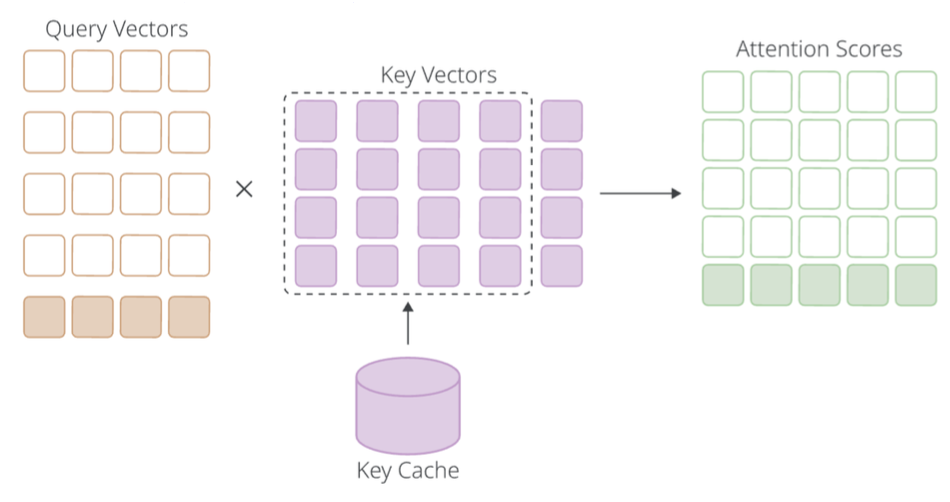
\includegraphics[width=0.9\textwidth]{figure/KVCache}
    \caption{Illustrazione del meccanismo KV Cache: i vettori query correnti vengono moltiplicati con i vettori key memorizzati nel cache per calcolare gli attention scores, evitando il ricalcolo delle rappresentazioni dei token precedenti.}
    \label{fig:KVC}
\end{figure}
\section{Multi Query Attention (MQA)}

La \textbf{MQA} (Multi Query Attention), introdotta nei modelli PaLM (Google) e Falcon, affronta il problema della memoria del KV Cache attraverso una strategia di condivisione delle rappresentazioni. L'idea fondamentale è quella di utilizzare un'unica coppia Key-Value condivisa tra tutte le teste di attenzione, mantenendo invece query separate per ogni testa:

\begin{align*}
Q_i &= h W_i^Q \quad \text{per } i = 1, \ldots, H \\
K &= h W^K \\
V &= h W^V
\end{align*}

dove $H$ è il numero di teste di attenzione, $h$ è la rappresentazione di input e $W_i^Q$, $W^K$, $W^V$ sono le matrici di proiezione.

\begin{figure}
    \centering
    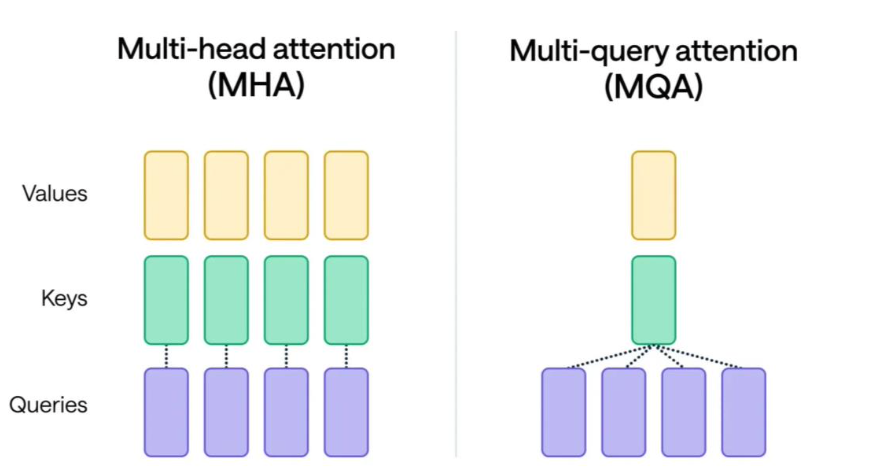
\includegraphics[width=0.9\textwidth]{figure/mha_vs_mqa_comparison.png}
    \caption{Architettura di Multi-Head Attention (MHA) vs Multi-Query Attention (MQA). MQA utilizza Key e Value condivisi tra tutte le teste di attenzione, mantenendo Query separate, riducendo così i requisiti di memoria del cache.}
    \label{fig:mha_vs_mqa}
\end{figure}

\subsection{Calcolo dell'Attenzione}
L'attenzione per ogni testa viene calcolata come:

\begin{equation}
    \text{head}_i = \text{Attention}(Q_i, K, V) = \text{softmax}\left(\frac{Q_i K^T}{\sqrt{d_k}}\right) V
\end{equation}

L'output finale è ottenuto concatenando tutte le teste:

\begin{equation}
    \text{MQA}(h) = \text{Concat}(\text{head}_1, \ldots, \text{head}_H) W^O
\end{equation}

\subsection{Riduzione della Memoria}
Con MQA, la dimensione del KV Cache diventa:

\begin{equation}
    \text{MQA Cache Size} = 2 \times \text{batch\_size} \times 1 \times \text{seq\_length} \times \text{head\_dim}
\end{equation}

Questo rappresenta una riduzione di un fattore $H$ (numero di teste) rispetto all'attenzione multi-head standard, risultando in significativi risparmi di memoria per modelli con molte teste di attenzione.

\subsection{Prestazioni}
Gli esperimenti mostrano che MQA mantiene prestazioni competitive rispetto all'attenzione multi-head standard, pur riducendo drasticamente i requisiti di memoria. Questo trade-off favorevole ha reso MQA una scelta popolare per modelli di grandi dimensioni.

\section{Grouped Query Attention (GQA)}

La \textbf{GQA} (Grouped Query Attention) invece, utilizzata in modelli come LLaMA 2~\cite{touvron2023llama}, LLaMA 3~\cite{touvron2024llama3} e Mistral 7B~\cite{mistral2023mistral7b}, rappresenta un compromesso tra Multi Head Attention standard e Multi Query Attention. Invece di utilizzare una singola coppia Key-Value per tutte le teste (MQA) o coppie separate per ogni testa (MHA), GQA organizza le teste in gruppi che condividono le stesse rappresentazioni Key-Value. Dato un numero totale di teste $H$ e un numero di gruppi $G$, ogni gruppo contiene $H/G$ teste di query che condividono la stessa coppia Key-Value:

\begin{align*}
    Q_{g,i} &= h W_{g,i}^Q \quad \text{per gruppo } g, \text{testa } i \\
    K_g &= h W_g^K \quad \text{per gruppo } g \\
    V_g &= h W_g^V \quad \text{per gruppo } g
\end{align*}

\subsection{Flessibilità della Configurazione}
GQA offre flessibilità nella scelta del numero di gruppi:
\begin{itemize}
\item $G = H$: equivale a Multi Head Attention standard;
\item $G = 1$: equivale a Multi Query Attention;
\item $1 < G < H$: compromesso ottimale tra prestazioni e efficienza.
\end{itemize}

\subsection{Dimensione del Cache}
La dimensione del KV Cache per GQA è:

\begin{equation}
\text{GQA Cache Size} = 2 \times \text{batch\_size} \times G \times \text{seq\_length} \times \text{head\_dim}
\end{equation}

dove $G$ è il numero di gruppi, fornendo una riduzione di memoria di un fattore $H/G$.
\begin{figure}
    \centering
    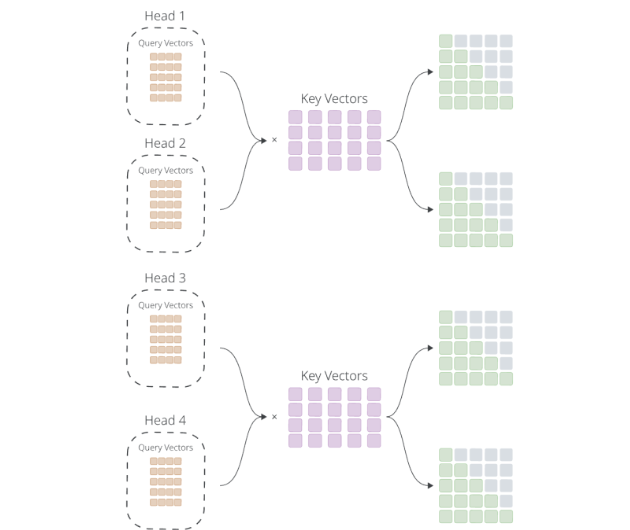
\includegraphics[width=0.7\textwidth]{figure/GPA.png}
    \caption{Architettura di un meccanismo di attenzione multi-head con quattro teste (Head 1-4). Ogni testa elabora un gruppo di Query Vectors in parallelo con Key Vectors, producendo matrici di attenzione indipendenti che possono essere successivamente combinate.}
    \label{fig:gpa}
\end{figure}
\subsection{Prestazioni}
GQA dimostra prestazioni superiori rispetto a MQA mantenendo significativi vantaggi in termini di memoria rispetto a MHA standard. Questa caratteristica l'ha resa una scelta preferita per molti modelli moderni di grandi dimensioni.

\section{Rotary Positional Embeddings}
Gli embeddings posizionali assoluti presentano diverse limitazioni, di seguito elenchiamo due degli aspetti princiapali per cui si definiscono abbastanza limitati:

\begin{itemize}
    \item \textbf{Lunghezza di Sequenza Limitata}: I modelli possono rappresentare posizioni solo fino a un limite predefinito durante l'addestramento, non potendo rappresentare posizioni oltre quel limite;
    \item \textbf{Indipendenza delle Posizioni}: Ogni embedding posizionale è indipendente dagli altri, questo comporta che nella visione del modello, la differenza fra la posizione 1 e la posizione 2 è la stessa che vi è fra la posizione 2 e la posizione 500, impedendo al modello di comprendere le relazioni relative tra posizioni.
\end{itemize}

La mancanza di posizionamento relativo può ostacolare la capacità del modello di comprendere la struttura linguistica, dove le relazioni tra parole dipendono spesso dalla loro distanza relativa piuttosto che dalle posizioni assolute. Gli embeddings posizionali relativi, come quelli utilizzati nel modello T5, si concentrano sulle distanze tra coppie di token piuttosto che sulle posizioni assolute. Tuttavia, presentano sfide pratiche:

\begin{itemize}
    \item \textbf{Problemi di Prestazioni}: Possono essere più lenti, specialmente per sequenze lunghe;
    \item \textbf{Complessità nel KV Cache}: Ogni token aggiuntivo altera l'embedding per tutti gli altri token, complicando l'uso efficiente del cache.
\end{itemize}

Proprio a queste complessità ingegneristiche, gli embedding posizionali non sono stati adottati largamente, spegialmente nel contesto le \textit{large language models}, differentemente dall'utilizzo di quelli rotazionali che vedremo in seguito, i quali si basano sulle \textit{matrici di rotazione}.

\subsection{Matrici di Rotazione}
Le \textbf{matrici di rotazione} costituiscono la base matematica di \textbf{RoPE}. Una matrice di rotazione 2D è definita come:

\begin{equation}
    R(\theta) = \begin{pmatrix}
    \cos\theta & -\sin\theta \\
    \sin\theta & \cos\theta
    \end{pmatrix}
\end{equation}

Quando questa matrice viene applicata a un vettore, tramite la moltiplicazione, questa matrice cambia l'angolo del vettore mantenendo invariata la sua lunghezza.

\subsection{Formulazione di RoPE}
Rotary Positional Embedding applica rotazioni position-dependent alle rappresentazioni query e key. Per due token alle posizioni $m$ e $n$:

\begin{align*}
    q_m &= R(\theta, m) \cdot W^Q h_m \\
    k_n &= R(\theta, n) \cdot W^K h_n
\end{align*}

dove $R(\theta, \operatorname{pos})$ è la matrice di rotazione dipendente dalla posizione, in questo caso rispettivamente l'ennesima ed emmesima posizione. Le matrici di rotazione possiedono la proprietà fondamentale:

\begin{equation}
    R(\theta, m)^T R(\theta, n) = R(\theta, n-m)
\end{equation}

Questa proprietà consente al prodotto scalare tra query e key di dipendere solo dalla loro distanza relativa $(n-m)$, ottenendo così un posizionamento relativo naturale. E questo torna utile nel momento in cui si vuole calcolare l'attention score come quanto segue, il quale grazie a questa proprietà subisce una trasformazione nel suo calcolo:

\begin{equation}
    \operatorname{score}= q_m\cdot k_n = q^TR_m^TR_nk = q^TR_{m-n}k
\end{equation}

Per concludere analizziamo i vantaggi che offre RoPE, i quali sono diversi rispetto agli embedding tradizionali che abbiamo sempre considerato:
\begin{itemize}
    \item \textbf{Posizionamento Relativo}: Intrinsecamente codifica le relazioni relative;
    \item \textbf{Lunghezza Flessibile}: Può gestire sequenze più lunghe di quelle viste durante l'addestramento;
    \item \textbf{Efficienza}: Compatibile con le tecniche di caching KV;
    \item \textbf{Adozione Diffusa}: Utilizzato in modelli come RoFormer~\cite{su2021roformer}, LLaMA 2~\cite{touvron2023llama}, LLaMA 3~\cite{touvron2024llama3}, Gemma~\cite{google2024gemma}, PaLM~\cite{chowdhery2022palm}, GPT-NeoX~\cite{black2022gptneox}, Falcon~\cite{penedo2023falcon}, DeepSeek V2~\cite{deepseek2023v2}, DeepSeek V3~\cite{deepseek2024v3}, DeepSeek R1~\cite{deepseek2024r1}.
\end{itemize}

\section{Multi Head Latent Attention (MLA)}

La \textbf{MLA} (Multi Head Latent Attention), è stata introdotta nei modelli DeepSeek V2, V3 e R1, rappresentando un approccio più avanzato per ridurre i requisiti di memoria del KV Cache. L'idea centrale è comprimere l'input dell'attenzione in uno spazio latente a bassa dimensionalità come visibile nella parte più a destra della Figura~\ref{fig:diffAttention}.


\begin{figure}
    \centering
    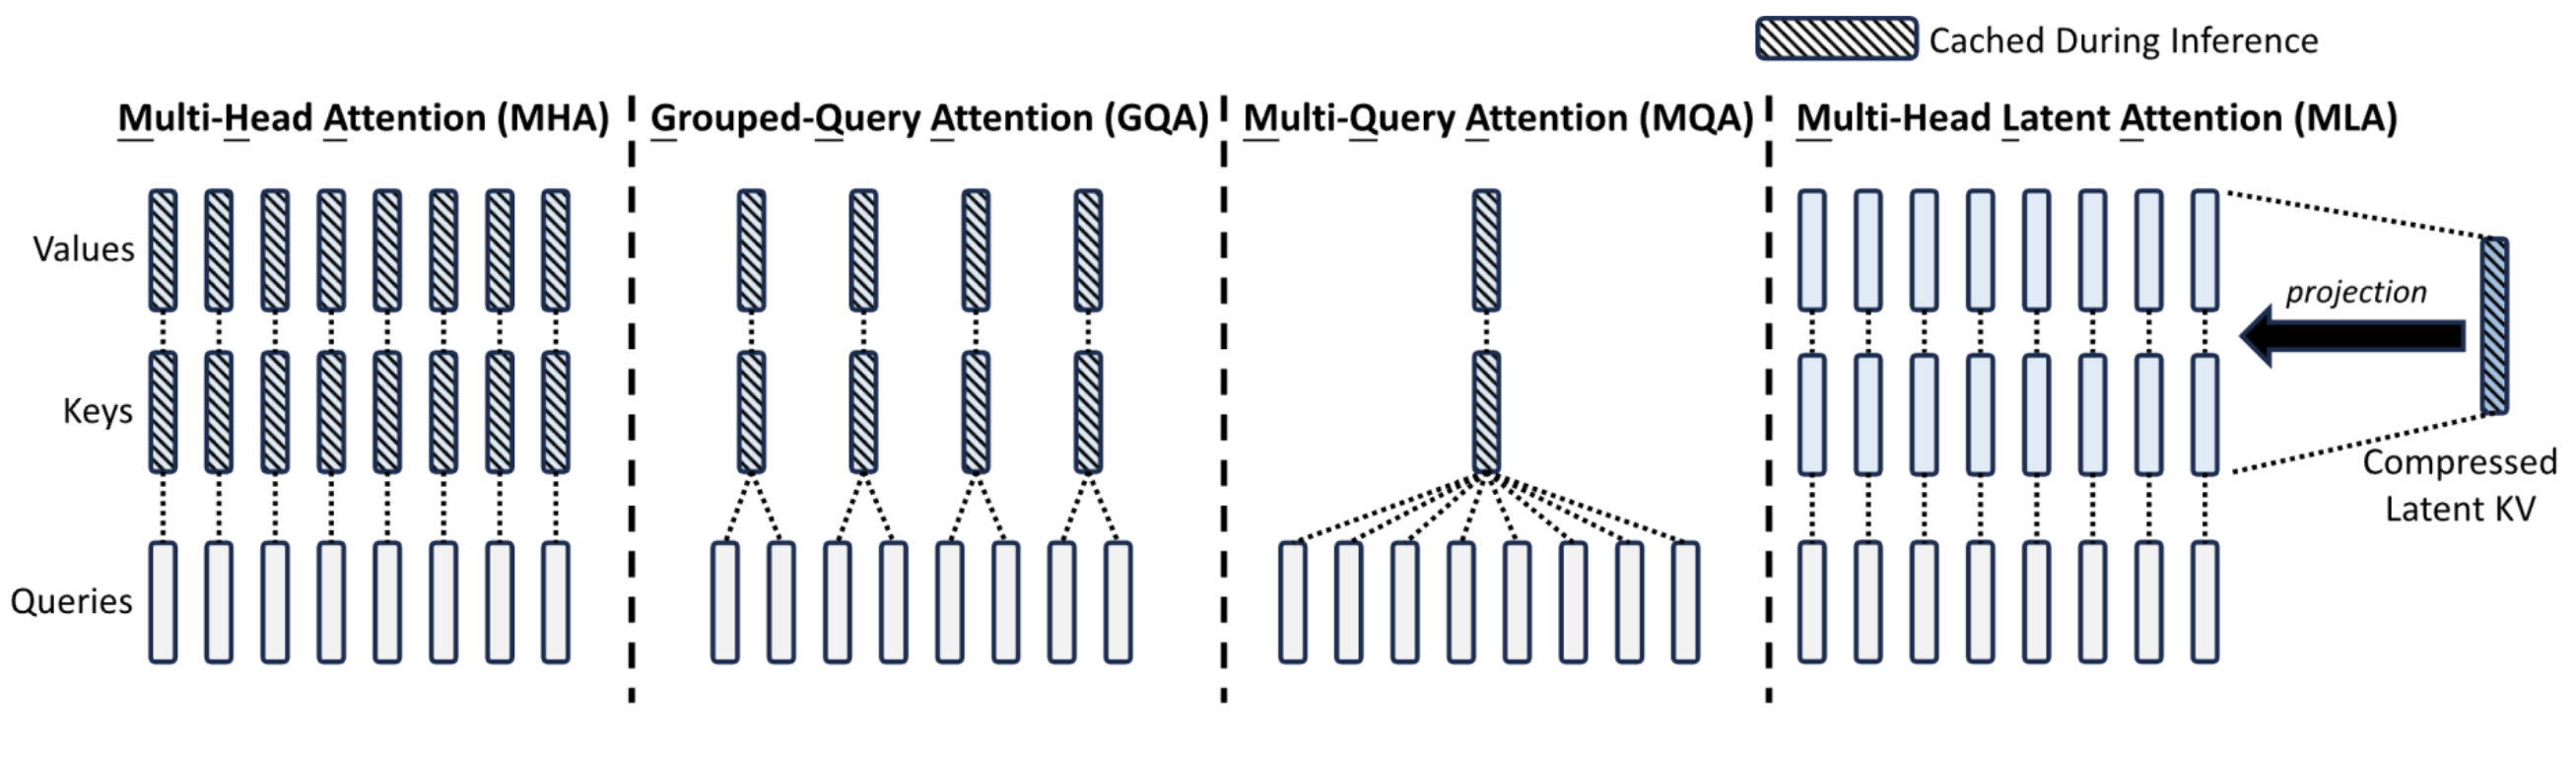
\includegraphics[width=\textwidth]{figure/DifferentAttention.png}
    \caption{Rappresentazioni dei diversi meccanismi dell'attenzione presentati in questo capitolo da sinistra verso destra: Multi Head Attention, Grouped Query Attention, Multi Query Attention e Multi-Head Latent Attention.}
    \label{fig:diffAttention}
\end{figure}

\subsection{Principio Fondamentale}
MLA comprime l'input dell'attenzione $h_t$ in un vettore latente a bassa dimensionalità $c_t^{KV}$ con dimensione $d_c$, dove $d_c \ll h_n \cdot d_h$:

\begin{equation}
    c_t^{KV} = W^{DKV}h_t
\end{equation}

dove $W^{DKV}$ è la matrice di compressione che riduce la dimensionalità da $(h_n \cdot d_h)$ a $d_c$.

\subsection{Recupero delle Chiavi e Valori}
Quando necessario per il calcolo dell'attenzione, il vettore latente viene mappato nuovamente nello spazio ad alta dimensionalità:

\begin{align*}
    K_t &= c_t^{KV} W^{UK} \\
    V_t &= c_t^{KV} W^{UV}
\end{align*}

dove $W^{UK}$ e $W^{UV}$ sono matrici di up-projection che mappano dallo spazio latente allo spazio originale.

\subsection{Trattamento delle Query}
Analogamente, le query possono essere trattate attraverso lo spazio latente:

\begin{align*}
    c_t^Q &= h_t W^{DQ} \\
    Q_t &= c_t^Q W^{UQ}
\end{align*}

\subsection{RoPE Disaccoppiato}
L'integrazione di RoPE con MLA presenta sfide tecniche. Nel caso standard, $W^{UK}$ può essere "assorbito" in $W^Q$, riducendo ulteriormente l'uso di memoria. Tuttavia, con RoPE, la matrice di rotazione position-dependent si interpone tra $(W^Q)^T$  e $W^{UK}$, impedendo questo assorbimento. Per risolvere questa problematica, MLA introduce il così chiamato "RoPE disaccoppiato":
\begin{itemize}
    \item Vettori query aggiuntivi vengono introdotti insieme a un vettore key condiviso;
    \item Questi vettori aggiuntivi sono utilizzati esclusivamente per il processo RoPE;
    \item Le chiavi originali rimangono isolate dalla matrice di rotazione.
\end{itemize}

\subsection{Calcolo dell'Attenzione MLA}
Il processo completo di calcolo dell'attenzione MLA include:

\begin{enumerate}
    \item Compressione dell'input nello spazio latente;
    \item Up-projection per recuperare keys e values;
    \item Applicazione del RoPE disaccoppiato;
    \item Calcolo dell'attenzione standard;
    \item Aggregazione dei risultati.
\end{enumerate}

\subsection{Riduzione della Memoria}
La dimensione del cache per MLA è drasticamente ridotta:

\begin{equation}
    \text{MLA Cache Size} = \text{batch\_size} \times \text{seq\_length} \times d_c
\end{equation}

dove $d_c$ è significativamente più piccolo della dimensione originale, risultando in riduzioni di memoria dell'ordine di grandezza.

\subsection{Prestazioni}
Gli esperimenti mostrano che MLA mantiene prestazioni competitive o superiori rispetto alle tecniche precedenti, pur ottenendo le maggiori riduzioni di memoria tra tutte le tecniche discusse. Questo ha reso MLA particolarmente attraente per modelli che devono gestire sequenze molto lunghe o operare con risorse computazionali limitate.

\section{Confronto delle Tecniche}

\subsection{Analisi Comparativa}
La tabella seguente riassume le caratteristiche principali delle diverse tecniche di attenzione:

\begin{table}[htbp]
    \centering
    \begin{adjustbox}{width=\textwidth}
    \begin{tabular}{|l|c|c|c|c|}
    \hline
    \textbf{Tecnica} & \textbf{Cache Size} & \textbf{Qualità} & \textbf{Complessità} & \textbf{Adozione} \\
    \hline
    Multi Head Attention & $2 \times B \times H \times L \times D$ & Alta & Bassa & Standard \\
    Multi Query Attention & $2 \times B \times 1 \times L \times D$ & Media & Bassa & Diffusa \\
    Grouped Query Attention & $2 \times B \times G \times L \times D$ & Alta & Bassa & Molto diffusa \\
    Multi Head Latent Attention & $B \times L \times d_c$ & Alta & Alta & Emergente \\
    \hline
    \end{tabular}
    \end{adjustbox}
    \caption{Confronto delle tecniche di attenzione avanzate}
    \label{tab:attention_comparison}
\end{table}

dove $B$ è la batch size, $H$ il numero di teste, $L$ la lunghezza della sequenza, $D$ la dimensione delle teste, $G$ il numero di gruppi, e $d_c$ la dimensione compressa.

\subsection{Scelta della Tecnica Ottimale}
La scelta della tecnica di attenzione dipende da diversi fattori:

\begin{itemize}
    \item \textbf{Risorse di Memoria}: MLA per limitazioni estreme, GQA per compromessi bilanciati;
    \item \textbf{Lunghezza delle Sequenze}: RoPE per sequenze lunghe, MLA per sequenze molto lunghe;
    \item \textbf{Prestazioni}: GQA per il miglior equilibrio prestazioni-efficienza;
    \item \textbf{Semplicità di Implementazione}: MQA per implementazioni rapide.
\end{itemize}

\section{Implementazioni Pratiche e Considerazioni}

L'implementazione efficiente di queste tecniche richiede considerazioni specifiche:

\begin{itemize}
    \item \textbf{Gestione della Memoria}: Allocazione dinamica del cache per sequenze di lunghezza variabile;
    \item \textbf{Parallelizzazione}: Ottimizzazione per GPU e TPU;
    \item \textbf{Precision}: Uso di mixed precision per ridurre ulteriormente l'uso di memoria;
    \item \textbf{Batch Processing}: Gestione efficiente di batch con sequenze di lunghezza diversa.
\end{itemize}

\subsection{Trade-off Prestazioni-Memoria}
Ogni tecnica presenta specifici trade-off:

\begin{description}
    \item[MQA] Massima semplicità implementativa con buone riduzioni di memoria
    \item[GQA] Miglior equilibrio tra prestazioni e efficienza
    \item[MLA] Massima riduzione di memoria con complessità implementativa maggiore
    \item[RoPE] Miglior gestione delle sequenze lunghe con overhead computazionale minimo
\end{description}

\section{Tendenze Future e Sviluppi}

Le direzioni future includono la così detta \textbf{Sparse Attention}, volta a ridurre la complessità quadratica dell'attenzione, l'\textbf{Adaptive Attention}, introducendo meccanismi che adattano la complessità alla difficoltà del task, avanzate tecniche di compressione più sofisticate per MLA, e ovviamente delle ottimizzazioni specifiche per le architetture hardware emergenti. Una cosa da considerare è come queste ottimizzazioni delle tecniche hanno permesso a modelli di diventare enormi quasi un trilione di parametri, garantire un inferenza efficiente su hardware dei consumatori, dare la possibilità di processare dei documenti molto lunghi e la possibilità infine di effettuare il deployment su dispositivi mobili, tutte non cose da poco. Le tecniche avanzate di attenzione multi-head rappresentano progressi fondamentali nell'ottimizzazione dei modelli Transformer. Dall'introduzione del KV Cache per accelerare l'inferenza, attraverso le varianti MQA e GQA per ridurre l'uso di memoria, fino agli embeddings posizionali rotatori per una migliore gestione delle sequenze lunghe e alla rivoluzionaria MLA per compressioni estreme, ogni innovazione ha contribuito a rendere i modelli di linguaggio di grandi dimensioni più pratici e accessibili. La scelta della tecnica ottimale dipende dai requisiti specifici dell'applicazione, dalle risorse disponibili e dai trade-off accettabili tra prestazioni e efficienza. Con il continuo sviluppo di nuove architetture e l'aumento delle dimensioni dei modelli, queste ottimizzazioni continueranno a evolversi, aprendo nuove possibilità per applicazioni sempre più sofisticate del deep learning nel processamento del linguaggio naturale. L'adozione diffusa di queste tecniche nei modelli moderni testimonia la loro efficacia e importanza pratica. Comprendere questi meccanismi è essenziale per chiunque lavori con modelli Transformer avanzati e rappresenta la base per future innovazioni nel campo.